This section describes the development platform and markup language that was chosen for the solution and the final design of the website. The final design is also presented and explained.

\subsection{ASP}
To make our solution easily available it was decided that it needed to be accessible through a browser. Since a specification requirement was that the program had to be written in C\# the obvious choice was building our application on the .ASP framework. ASP.NET is a server-side Web application framework. This means that the majority of the code is executed on the server rather than on the client machine. In an ASP.NET application you need to execute code on the client side. For instance to check certain conditions before executing resource heavy code on the server. This can be done through Javascript or JQuery. There are numerous advantages to using the ASP.NET framework. For example, it takes care of almost all of the threading and networking. While we have made our data-structures protected against multi-threading, we have not been able to actually test our application with multiple-users. We made our data-structure protected by using a singleton structure which limits an object to never be instantiated more than onceand instead returns the one instance.

Because all of the code is run server-side and you can manipulate designated html-elements  (designated with the <asp:”...”> tag), it is simple to make our website dynamic and user friendly. An example of making the website dynamic, is in the preference tab when the user changes his preferences the CheckBoxList object has a C\# event handler, so that when anything in that object changes the appropriate changes are made on the server.

\subsection{Final design}
The design of the website got changed because we wanted to give it a simple and fitting design. As seen on Figure \ref{fig:new-login} and Figure \ref{fig:new-signup} you can see that the colour and design have been changed a lot compared to the previous login design, which can be seen in Figure \ref{Login} on page \pageref{Login}. In the previous version there no any signup feature. This signup feature only does the basics, like username, password, gender, and date of birth. The colour black was chosen for the background as it blends well with blue and white. The colour black and white gives, according to Figure \ref{Colors} on page \pageref{Colors}, a sense of neutrality and the colour blue gives a sense of calm and neutrality. According to Judy Scott-Kemmis \cite{EmpowerColor}, the meaming of black is the secretive and the unknown, white is the colour of perfection, and blue is the colour of trust and peace. Black, white and blue is the basic colours that was used for the GUI design.


\begin{figure}[H]
\centering
\begin{subfigure}{.5\textwidth}
  \centering
  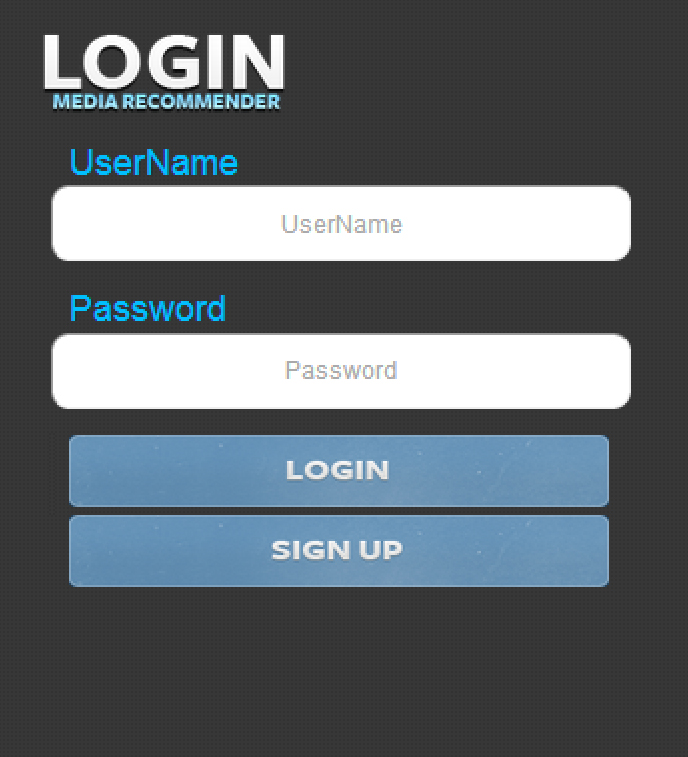
\includegraphics[width=.9\linewidth]{Images/new-login.jpg}
  \caption{Login}
  \label{fig:new-login}
\end{subfigure}%
\begin{subfigure}{.5\textwidth}
  \centering
  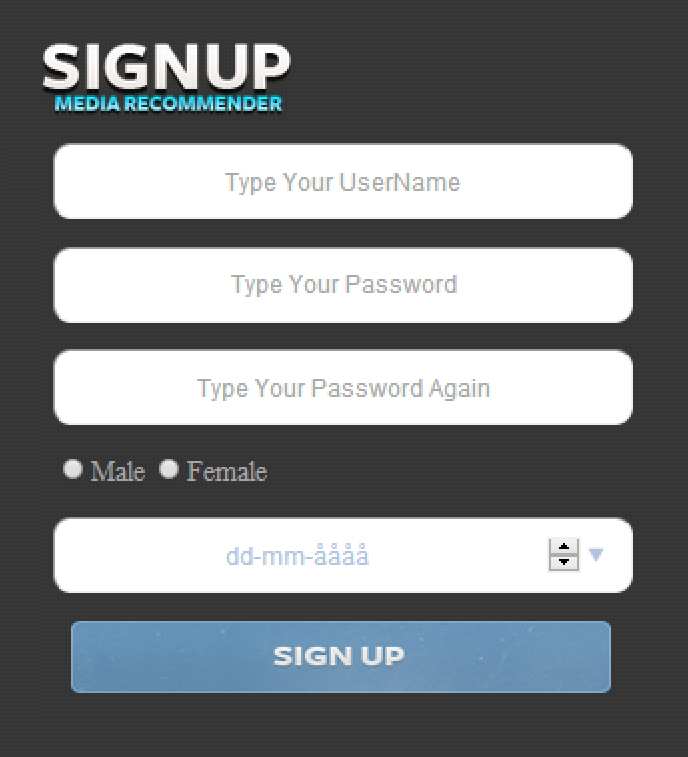
\includegraphics[width=.9\linewidth]{Images/new-signup.jpg}
  \caption{Signup}
  \label{fig:new-signup}
\end{subfigure}
\caption{Redesign of Login and Signup}
\label{fig:login-signup}
\end{figure}



After creating a user and logging in to the website you are directed to the frontpage. Compared to the old design of the website, as seen in Figure \ref{CurrSite} on page \pageref{CurrSite}, there has been added a search bar and the ability to specify which rating you want to give to each media. By hitting enter after writing something into the search bar, the search will be done, instead of having to do it manually with a button click. The rating is made out of radio buttons from 0 to 10, which makes it convenient for the user when he wants to indicate a rating for a media. Every rating is displayed on the medialist tab in the form of stars. The 0 to 10 rating system is converted into a 0 to 5 star system, where a rating of 1 is half a star, and a rating of 5 is two and a half star.

As seen on Figure \ref{fig:new-frontpage} you can see that movies, games, and books have been combined into one button called "Recommendation", when compared to the old design seen on Figure \ref{CurrSite} on page \pageref{CurrSite}. The recommendation button was chosen to be red since according to Figure \ref{Colors} it gives a sense of what is hot, and according to \cite{EmpowerColor} it means that you are ready to take action. If you rate and add a media to your medialist it will give you a notification saying “Added to your medialist”, so the user will know where his media will be added to. This is not the most optimal way, since you will not know from the beginning that you can click on the media and it will be added to your medialist. This feature would have to be made more obvious

\begin{figure}[H]
\centering
\begin{subfigure}{.5\textwidth}
  \centering
  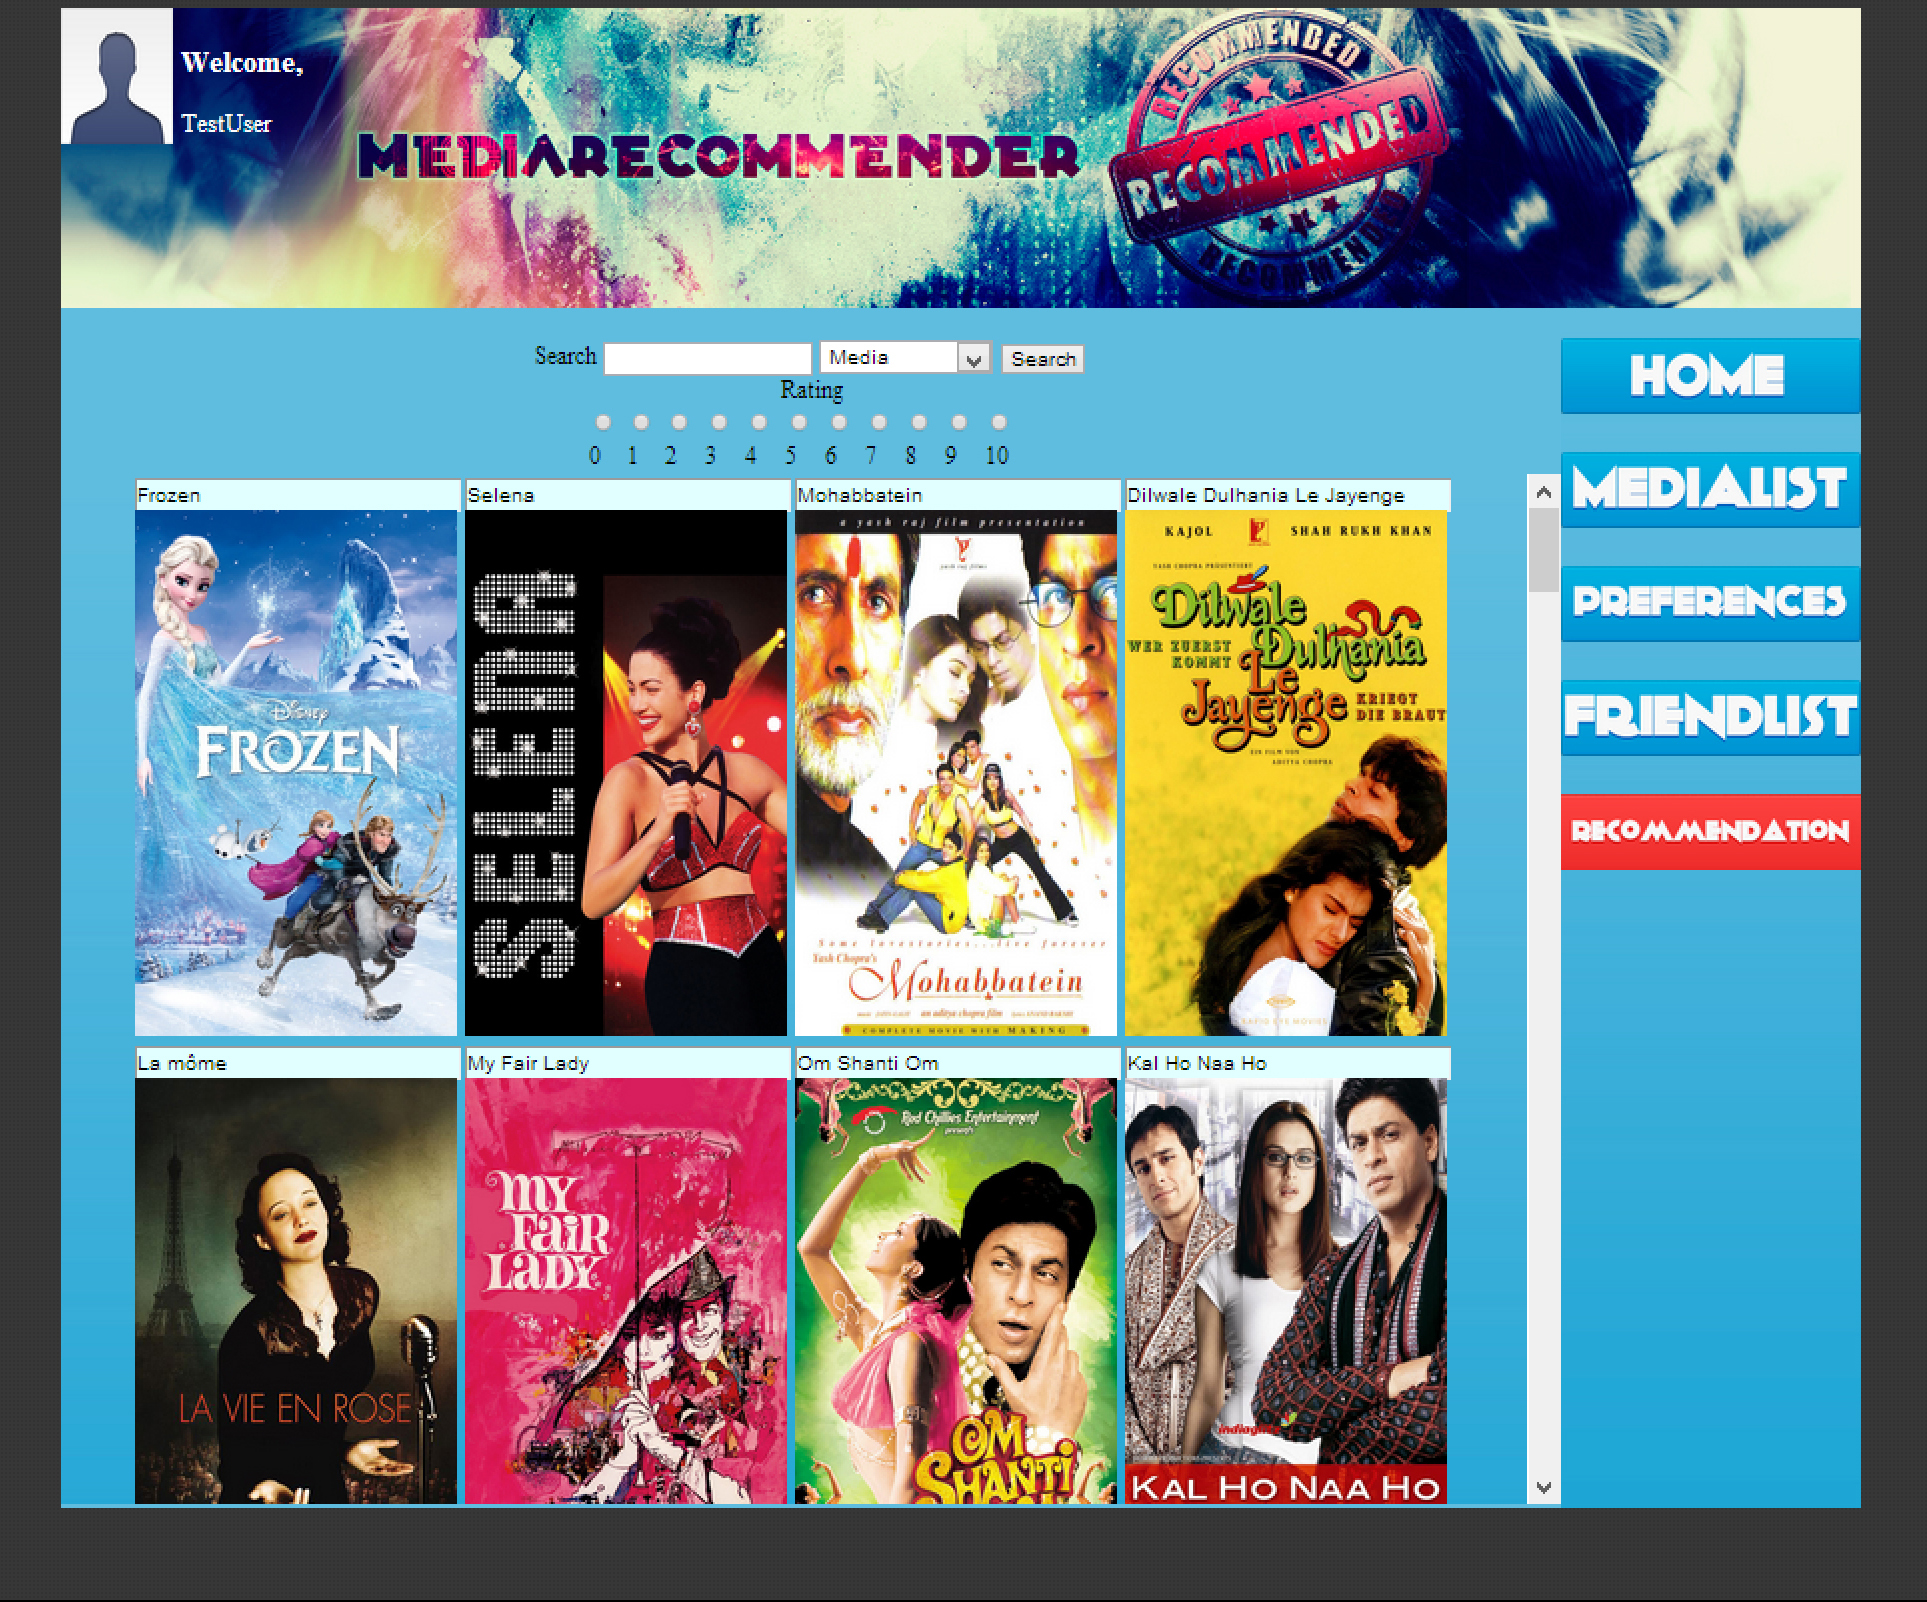
\includegraphics[width=.9\linewidth]{Images/new-home.jpg}
  \caption{Frontpage}
  \label{fig:new-frontpage}
\end{subfigure}%
\begin{subfigure}{.5\textwidth}
  \centering
  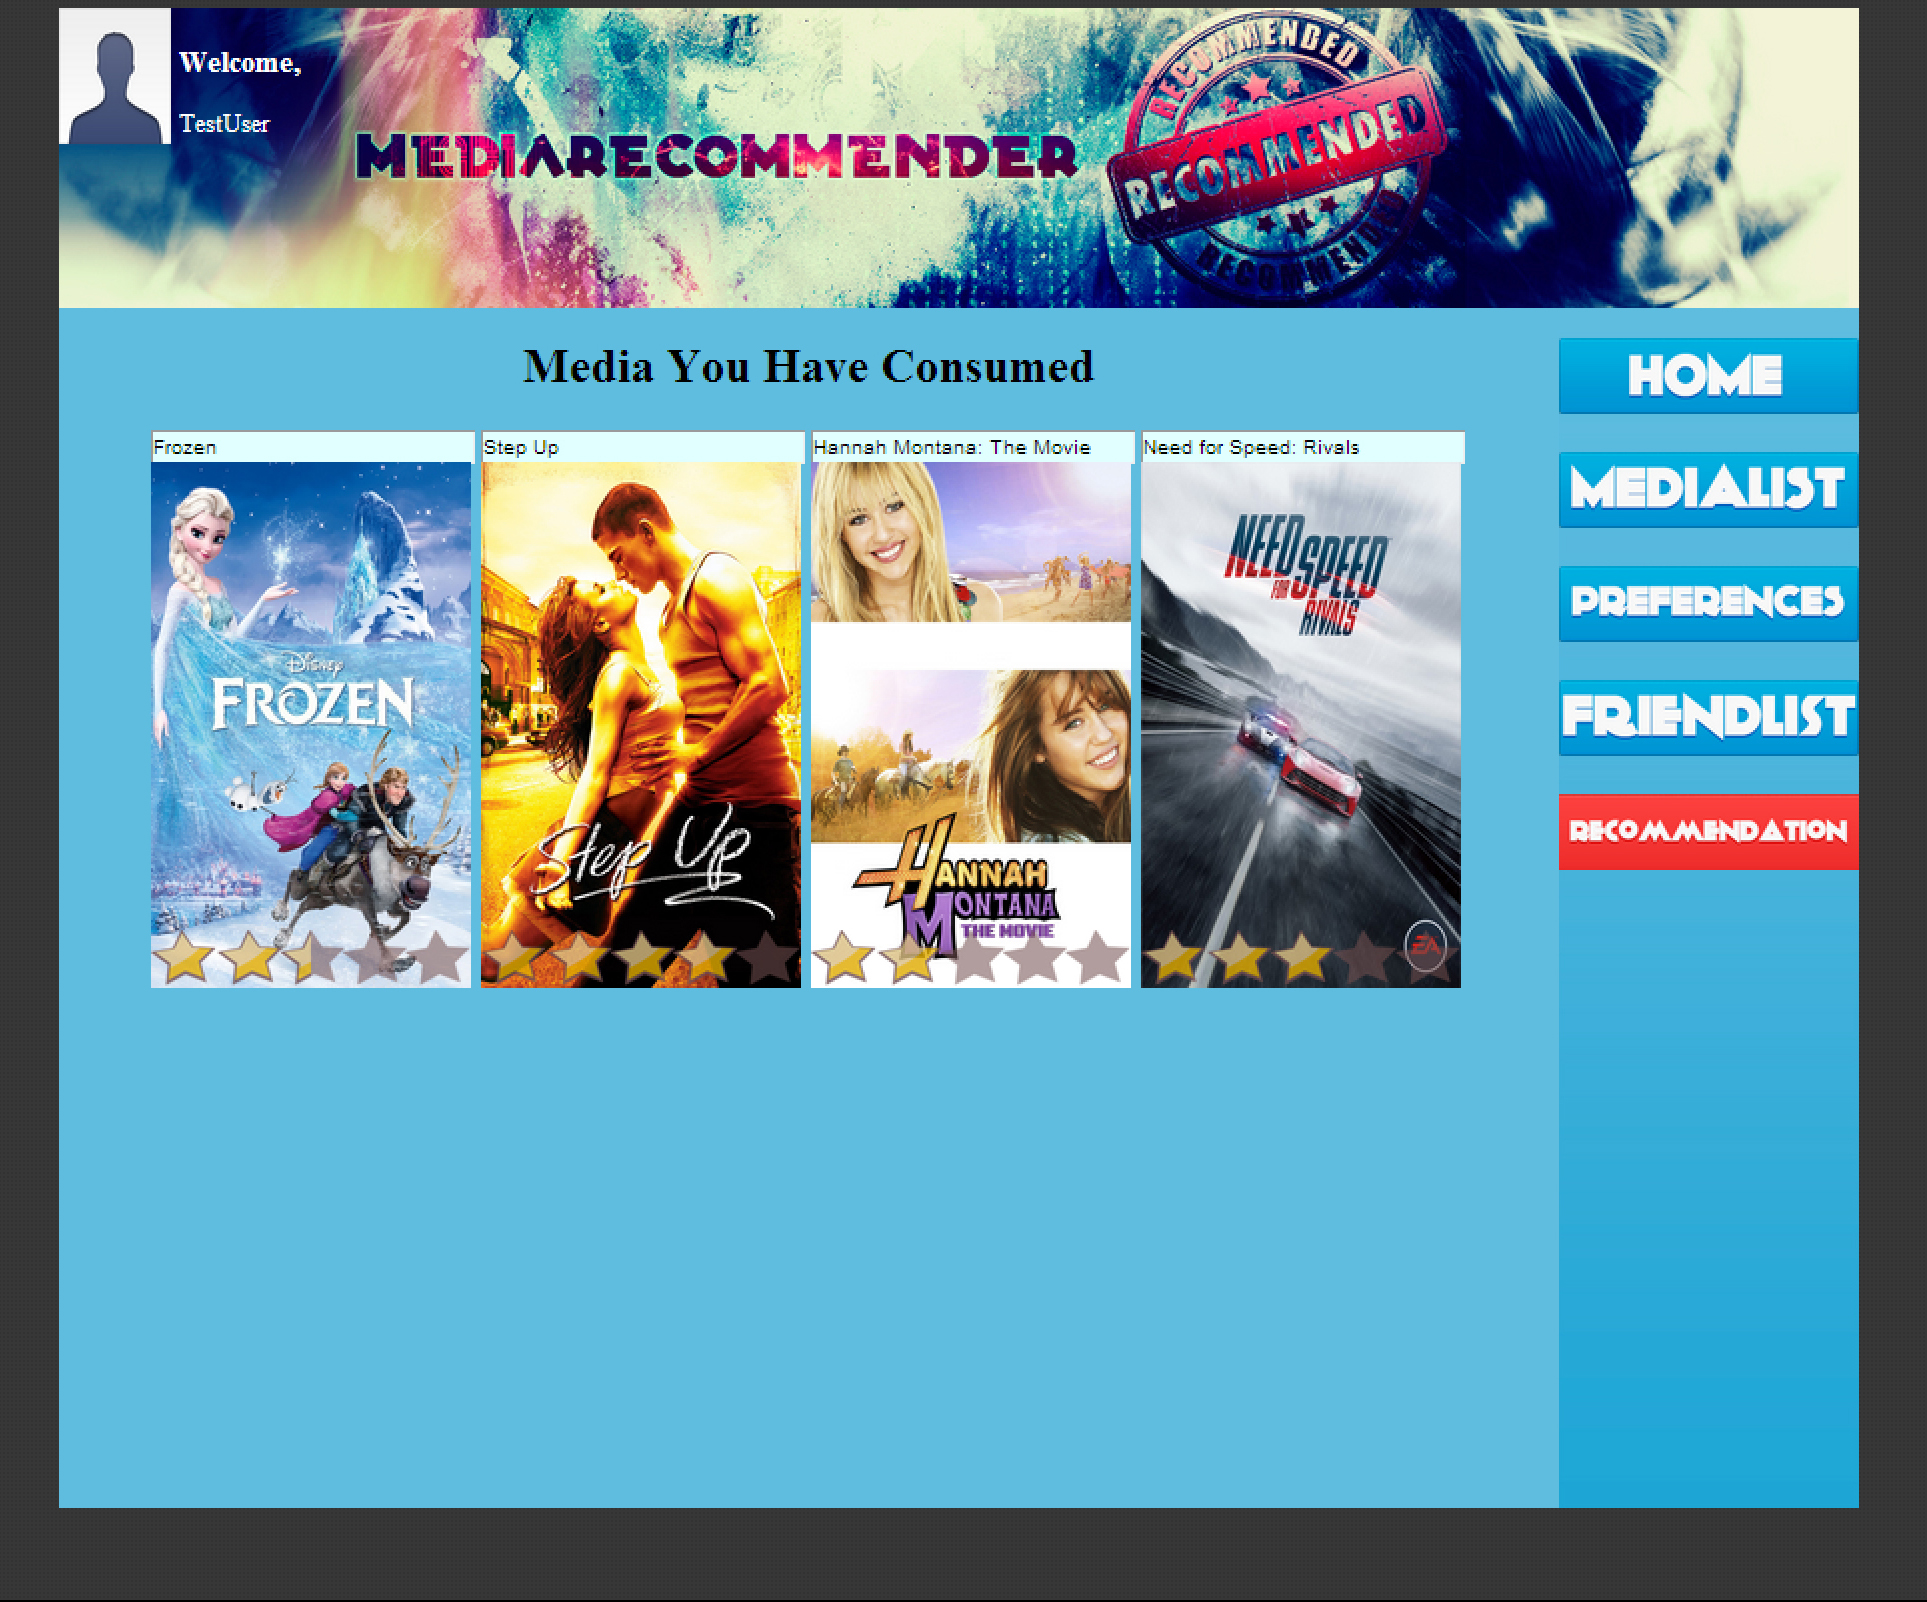
\includegraphics[width=.9\linewidth]{Images/new-medialist.jpg}
  \caption{Medialist}
  \label{fig:new-medialist}
\end{subfigure}
\caption{Redesign of frontpage and medialist}
\label{fig:front-media}
\end{figure}

The medialist page, as seen on Figure \ref{fig:new-medialist}, you will see all the media you have added to your medialist and their corresponding rating shown on the cover as stars. If you click on the media a confirmation notification is shown, saying “Are you sure you want to remove this media?”. Depending on the users' answer the media will be removed from the users' medialist. Again this is not the optimal way to do it, because there is no way for the user to know this beforehand. This feature would also have to be made obvious

The preference page is where all the genres available to the system appears. The user can specify what genres he prefers. What the user chooses here affects the outcome of the recommendation algorithm. The recommendation page is where the user gets his recommendations done by the collaborative and content-based hybrid algorithms. The output of the algorithm is shown in containers, one for each media item. The design still uses neutral colors, white, blue, and black, to cater to the target audience, and making the user of the system more comfortable.